%Schriftgröße, Layout, Papierformat, Art des Dokumentes
\documentclass[11pt,oneside,a4paper,titlepage]{article}
%Einstellungen der Seitenränder
\usepackage[inner=3.0cm,outer=2.5cm,top=2.5cm,bottom=2.5cm]{geometry}
\usepackage[ngerman]{babel}
\usepackage[utf8]{inputenc}
% wegen "lastchecked"
\usepackage{url}
% hyperref mit sinnvollen einstellungen
\usepackage[pdftex,
        colorlinks=true,
        urlcolor=black,                       % \href{...}{...} external (URL)
        filecolor=black,                      % \href{...} local file
        linkcolor=black,                      % \ref{...} and \pageref{...}
        citecolor=black,
        pdfauthor={Gruppe 2},
        pdfkeywords={},
        pdfproducer={pdfLaTeX},
    	%pdfadjustspacing=1,
        plainpages=false,
        pdfpagelabels,
        pagebackref,
        pdfpagemode=UseOutlines,
        pdfstartview={FitV},
        bookmarksopenlevel=section,
        bookmarksopen=false]{hyperref} 
% meist verwendetes Grafik-Paket
\usepackage{graphicx}
%\usepackage[authoryear]{natbib}
% weitere Pakete
\usepackage{subfig}
\usepackage{amsmath}
\usepackage{amssymb}
\usepackage{setspace}
\usepackage{url}
\usepackage{listings}
\usepackage{algorithm}
\usepackage{algorithmic}
\usepackage{color}
\usepackage{verbatim,framed} 
\usepackage{booktabs}
\usepackage{tabularx}
\usepackage{lipsum}
\usepackage{hyperref}
\usepackage[figure]{hypcap}
\usepackage{subfig}

\raggedbottom %Allow end of pages to be emtpy after pagebreak

\onehalfspacing %1.5-facher zeilenabstand

%Kopf- und Fußzeile
\usepackage{fancyhdr}
\fancyhf{}

% Informationen zur Arbeit
\title{{SysAd Projekt Roboter Orchestrierungssoftware}}
\author{Stefan Geiring, Marvin Müller, Nicolas Baumgärtner}
\date{Jan 21th, 2023}

%\setcitestyle{square}

\setcounter{secnumdepth}{3}

\begin{document}

% no indent
\setlength{\parindent}{0pt}

% Einbinden der Titelseite
\pagestyle{empty}

%\begin{flushright}
%
\includegraphics[scale=0.1]{imgs/rwu_logo.png}
%\end{flushright}


\begin{center}


\vspace*{2cm}

\includegraphics[scale=0.15]{imgs/rwu_logo.png}
\vspace*{3cm}

\huge
\textbf{Roboter Orchestrierungssoftware}\\
\Large
\vspace*{2cm}
\noindent \textbf{Expos\'e für die Lehrveranstaltung Systemadministration}\\
\vspace*{0.5cm}
\noindent \textbf{Stefan Geiring, ???}\\
\noindent \textbf{Marvin Müller, 32850}\\
\noindent \textbf{Nicolas Baumgärtner, 32849}\\
\vspace*{0.5cm}
Wintersemester 22/23\\
\normalsize 
05.November 2022
\vspace*{2cm}
\end{center}


\vspace*{4.5cm}
\begin{tabular}{ll}
Betreuer: & M.Sc. Aykan D. Inan \\
 & Ravensburg-Weingarten University of Applied Sciences\\
\end{tabular}



% Seitenstil

%Kopfzeile kapitel außen
%\fancyhead[RO,LE]{Abstract}


\newpage

\pagestyle{fancy}
%\pagestyle{empty}
%\cleardoublepage{}
%\pagestyle{fancy}

% titel/inhaltsverzeichnis

\fancyhead[RO,LE]{Contents}
\tableofcontents

\fancyhead[RO,LE]{\nouppercase{\leftmark}}
\fancyfoot[RO,LE]{\thepage}

%Linie oben
\renewcommand{\headrulewidth}{0.5pt}

% Zähler für Seiten
\setcounter{page}{1}

\newpage

% BEGINN INHALT **************************************************************

% \section{Einleitung}

\section{Thema}
\begin{flushleft}
    Entwicklung einer Orchestrierungssoftware mit Weboberfläche auf Basis von ROS.

    Roboter werden immer häufiger eingesetzt egal ob in Spezial Industrial bereichen oder auch einfach zuhause.
    Die einfache und übersichtliche Orchestrierung vieler Roboter ist deshalb besonders wichtig.
    Roboter Schwärme spielen außerdem, in der heutigen Zeit immer öfters eine wichtige Rolle.
    Ein Beispiel für große Roboter Schwärme die bereits eingesetzt werden sind Lieferdrohen, Drohnenshows als 
    ersatz für Feuerwerk oder die simplere Variante davon, eine Lagerverwaltung.
\end{flushleft}

\section{Motivation}
\begin{flushleft}
    Die Hauptmotivation für dieses Projekt besteht darin weitere Teile des ROS-Oekosystems neben dem standardmäßigen ROS1 kennenzulernen.
    
    Das bietet die Möglichkeit der Aneignung neuen Wissens in einem fächerübergreifenden Projekt, das sich über 4 Sektoren: der reinen Softwareentwicklung,
    Webentwicklung, Hardware/Elektronik-Entwicklung als auch der Robotik Entwicklung/Forschung erstreckt.\\

    Neben der reinen Aneignung von Wissen soll es uns aber auch die Möglichkeit geben weitere Projekte in Zukunft auf diesem Wissen aufzubauen und gemeinsam mit dem Robotiklabor der Hochschule neue Projekte zu erstellen.
\end{flushleft}

\section{Ziel}
\begin{flushleft}
    Ziel des Projektes soll es sein eine
    Orchestrierungssoftware für Roboter auf ROS2 Basis zu entwicklen.
    Mit der Hilfe der Orchestrierungssoftware soll es möglich sein, die Roboter zu überwachen und zu steuern.

    Desweitern soll eine Hardware Platform für einen kleinen Beispiel Roboter entwickelt werden, welche im
    nachhinein durch diverse Komponenten erweitert werden können. Wie zum Beispiel Kamera, Bumper, Laser etc.
\end{flushleft}

\section{Eigene Leistung}
\begin{flushleft}

    Ein bedeutender Teil unserer eigenen Leistung ist die Entwickung einer einfachen Weboberfläche auf ROS Basis welche als
    Orchestrierungssoftware für Roboter dienen soll.
    Die Weboberfläche der Orchestrierungssoftware soll in erster Linie als einfache Kontroll- und Debugging-Schnittstele dienen.
    
    Um unsere Orchestrierungssoftware sinngemäß demonstrieren zu können sollen außerdem kleine Roboter auf
    ESP32 Basis gebaut werden. Diese Roboter sollen aus einem 3D-Gedruckten Gehäuse bestehen.
    Auf den ESP32 soll Micro-ROS auf Basis von FreeRTOS ausgeführt werden.

    Unsere kleinen Beispiel-Roboter sollen außerdem im Idealfall mit modular austauschbaren Erweiterungen ausstattbar sein.
    Diese Erweiterungen sollen Simple Sensorik und Aktorik zur Verfügung stellen.
\end{flushleft}

\section{Aufbau der Arbeit}
\begin{flushleft}
    Gliederung:
    \begin{enumerate}
    \item Einleitung
    \begin{enumerate}
        \item Motivation
        \item Ziel
        \item Eigene Leistung
        \item Aufbau der Arbeit
    \end{enumerate}
    \item Grundbegriffe (Anhang)
    \item Zielsetzung und Anforderungen
    \item Stand der Technik und Forschung
    \item Lösungsideen
    \item Evaluation der Lösungsideen anhand der Anforderungen
    \item Implementierung
    \item Evaluation der Implementierung
    \item Fazit und Ausblick
    \end{enumerate}
\end{flushleft}
\pagebreak

\section{Grundbegriffe}
\begin{flushleft}
    \begin{description}
        \item[Docker:]\hfill\\
        Software für die Container Verwaltung.

        \item[ROS:]\hfill\\
        Das Acronym ROS steht für Robot Operating System, es bietet eine Sammlung von Software-Bibliotheken, Werkzeugen und ein Framework um die Softwareentwicklung und Ausführung von Andwendugen für Roboter zu erleichtern. \cite{ros}

        \item[React:]\hfill\\
        Web Frontend Framework was ursprünglich von Facebook ins leben gerufen wurde um deklarativ und Komponentenbasiert User-Interfaces zu entwickeln. \cite{reactframework}

        \item[Arduino:]\hfill\\
        Entwicklungsplatform auf Basis von Atmel AtMega Prozessoren. Wurde entworfen um Leien den Einstieg in die Microcontroller
        Welt stark zu vereinfachen. Findet heutzutage weltweit Anwendung in der Maker Szene. \cite{arduino}

        \item[ESP32:]\hfill\\
        ESP32 bezeichnet eine Microntroller Familie auf Basis der ARM Architektur.
        Die ESP32-Familie wurde von der Firma Espressif entwickelt. \cite{esp32}

        \item[RaspberryPi:]\hfill\\
        Single-board Computer der Raspberry Foundation. Der Computer wurde entwickelt um vor allem Kindern das Programmieren und Arbeiten mit Computern näher zu bringen.
        Raspberry pis werden außerdem häufig für Hobby-IOT und Robotikprojekte auf Grund der geringen Kosten im Verhätnis zur Konnektivität und Rechenleistung.\cite{raspberry_pi}
        
        \item[ESP-IDF:]\hfill\\
        ESP-IDF steht für Espressif IOT Development Framework. Das ist ein Framework mit dessen Hilfe man ESP-Socs programmieren kann. \cite{esp_idf}
        
        \item[RTOS]\hfill\\
        Abkürzung für Real Time Operating System. 
        In diesem Projekt wurde in erster Linie das RTOS 'FreeRTOS' verwendet, das für die Verwendung mit Mikrocontrollern optimiert ist. \cite{freertos}
        
        \item[Micro-ROS:]\hfill\\
        Micro-ROS wird ein Framework genannt welches es ermöglicht Mikrocontroller in das ROS Oekosystem einzubinden.
        Mehr dazu im Kapitel Stand der Technik und Forschung. (TODO: LINK?)

        \item[Toolchain:] \hfill\\
        Eine Toolchain ist eine Kombination mehrerer Softwaretools um komplexe Aufgaben in der Software Entwicklung durchzuführen.
        In speziellen Fall dieser Arbeit ist es eine Kombination von Micro-ROS und ESP-IDF.
        Mit Hilfe dieser Tools wird die Software für den Roboter cross-compiliert, geflasht und konfiguriert. \cite{micro_ros}

        \end{description}
\end{flushleft}
\pagebreak

\section{Zielsetzung und Anforderungen}
\begin{flushleft}
    Entwicklung einer Weboberfläche mit der Roboter aus ROS basis gesteuert und überwacht werden können.
    Oberfläche zeigt alle Roboter an und stellt Basic tools zur verfügung um mit diesen zu kommunizieren
    und diese zu steuern.
    Außerdem soll eine Schnittstelle zwischen Web und ROS geschaffen werden.

    (evtl. als diagram)

    Kosten:
    \begin{itemize}
    \item Endkosten belaufen sich auf weniger als 100€.
    \item In diesen Kosten soll der Microcontroller inkl. 3D-Druck und gesamter Elektronik inkludiert sein.
    \end{itemize}

    Leistung:
    \begin{itemize}
    \item Weboberfläche ist lauffähig.
    \item Roboter kann mit ROS-Messages gesteuert werden.
    \item In Eigenleistung kleine fahrbare Roboterplatform auf ESP32 basis kreieren.
    \end{itemize}
        
    Zu vermeiden:
    \begin{itemize}
    \item Keinen zu komplexen Roboter designen. (Vollständig autonom fahrender Roboter)
    \item Feature creep mit all zu vielen Sensoren gilt zu vermeiden.
    \item Roboter Antrieb mit zu viel Technik ausstatten.
    \item Vorerst sollte nur ein Testroboter entwicklet werden.
    \item Webinterface nicht zu stark mit ROS Datentypen befüllen.
    \end {itemize}

    Termine:
    \begin{itemize}
    \item 20.11. Abgabe Gamma Version.
    \item 23.12. Abgabe Beta Version.
    \item 30.12. Feedback zu Beta Versionen.
    \item 21.01. Finale Abgabe.
    \end{itemize}
    
\end{flushleft}

\section{Stand der Technik und Forschung}
\begin{flushleft}
    \textit{Technologischer Standpunkt Software:}\\
    (TODO React???)
    ROS bietet bereits ein starkes und recht einfach nutzbares Framework, allerdings vermisst man eine 
    schöne und einfach bedienbare graphische Oberfläche.
    Es existieren kleinere Projekte welche sich dieser Frontend entwicklung annehmen. 
    Allerdings hat uns keines dieser Projekte zufrieden gestellt. 
    Vor allem was die Orchestrierungsmöglichkeit mehrerer Roboter angeht.

    \begin{description}
        \item[Robotik:]\hfill\\
        \begin{flushleft}
    Ganz klar werden hier die Begriffe \textit{Roboter} und \textit{Robotik} voneinander getrennt.
    Wo der Begriff \textit{Roboter} klar definiert ist und unter strengen Richtlinien und Normen steht, die beschreiben, was ein Roboter ist, da ist der Begriff der \textit{Robotik} nicht genau definiert.
    
    Jedoch versteht man in der Robotik die Steuerung und Anwendung von Robotersystemen.
    Ganz gleich können hier Industrie- und Serviceroboter mit in Verbindung gebracht werden.
    Ein wichtiges Merkmal hierfür ist die Interaktion mit der physischen Welt, wofür ein Roboter Aktoren und Sensoren benutzt.
    Die Robotik ist eine interdisziplinäre Wissenschaft, da sie Gebiete der Informatik, Maschinenbau, Elektronik und der Mathematik vereint. 
    \cite{robotik_konradin}

    Als eines des bekanntesten und meist verbreitetsten Frameworks zur Steuerung von Robotern ist ROS (Robot Operating System), auf das im Folgenden Kapitel der Grundbegriffe genauer eingegangen wird.

\end{flushleft}

        \item[ROS:]\hfill\\
        ROS steht für Robot Operating System. Das "Operating System" ist kein richtiges Betriebssystem sondern eine Sammlung von Softwarebibliotheken, die es einem vereinfachen Robotiksysteme zu bauen.
        Der Kern von ROS besteht aus Interfaces, genannt ROS-Graph, die eine anonymisierte und standardisierte Interprozesskommunikation ermöglichen.
        Dieser Graph ist ein Netzwerk aus 'nodes', welche über 'topics' miteinander kommunizieren. 'Nodes' werden als Prozesse auf einem oder verschiedenen Computern ausgeführt.
        Auf einem 'topic' wird immer dieselbe 'message' mit einem definierten Datentyp von 'nodes' verbreitet. 
        Für das Verbreiten und Empfangen von Messages müssen die Nodes 'publisher' und 'subscriber'-Interfaces implementieren.
        In Abbildung \ref{fig:ros_graph} kann man einen ROS-Graph sehen, der aus zwei Nodes besteht, die über ein Topic miteinander kommunizieren.
        In diesem Fall gibt es einen publisher der Nachrichten sendet und einen subscriber der Nachrichten empfangen kann.

        \begin{figure}[h!]
            \centering
            
\includegraphics[width=0.8\textwidth]{imgs/Grundbegriffe/graph_2_nodes_with_topic.png}
            \caption{Beispiel ROS Graph}
            \label{fig:ros_graph}%
        \end{figure}

        Des weiteren gibt es noch viele Tools, die wie zum Beispiel in Abbildung \ref{fig:ros_graph} den ROS-Graph visualisieren können, und eine große Menge an Bibliotheken, welche Standard-Algorithmen der Robotik implementieren.
        Diese Tools und Bibliotheken werden ebenfalls zu ROS gezählt weshalb ROS als mehr als ein Framework angesehen wird.

        Es gibt eine ältere Version von ROS die einfach nur ROS genannt wird und eine neuere Version namens ROS2.
        Der Hauptunterschied zwischen ROS und ROS2 ist, dass ROS einen zentralen Server, genannt 'ROS-Master' verwendet und ROS2 einen dezentralen Ansatz verfolgt.
        Der 'ROS-Master' besteht im Kern aus einer Datenbank in der die Teilnehmer der verschiedenen Topics aufgelistet werden und in der die Teilnehmer des Netzwerks ihre entsprechenden Partner finden können, mit denen sie eine TCP-Verbindung aufbauen.
        
        ROS2 baut auf dem Data-Distribution Service Standard von OMG auf. 
        Das ist eine Spezifikation für eine Middleware, welche ein 'Data-Centric Subscriber-Publisher (DCPS)'-Modell beschreibt und somit sehr ähnlich zu dem ROS-Graphen ist. 
        Die Middleware stellt die Peer-to-Peer Funktionalität auf Basis von UDP zur Verfügung.

        \item[Micro-ROS]\hfill\\
        Micro-ROS ist eine Kombination von einem RTOS, einer Client-Bibliothek, einer Middleware und einem sogenannten ROS2 Agent, 
        die Mikrocontroller möglichst effizient in das ROS-Oekosystem einbinden soll.
        
        Mit Micro-ROS ist es nicht möglich ROS-messages direkt im Netzwerk zu versenden und mit anderen Teilnehmern direkt in Verbindung zu stehen.
        Die dafür benötigte Middleware würde zu viele Ressourcen auf einem Mikrocontroller verbrauchen. 
        Stattdessen gibt es einen sogenannten ROS-Agent, mit dem sich der Mikrocontroller mit Hilfe einer für Mikrocontroller optimierten Middleware verbindet.
        Der ROS-Agent ist dann im Prinzip eine Brücke zwischen den verschiedenen Middlewares, wie man in Abbildung \ref{fig:micro-ros-architecture} sehen kann. Entsprechend muss der Agent auch auf leistungsfähigerer Hardware ausgeführt werden.    
        \cite{micro_ros_concepts}
        \begin{figure}[h!]
            \centering
            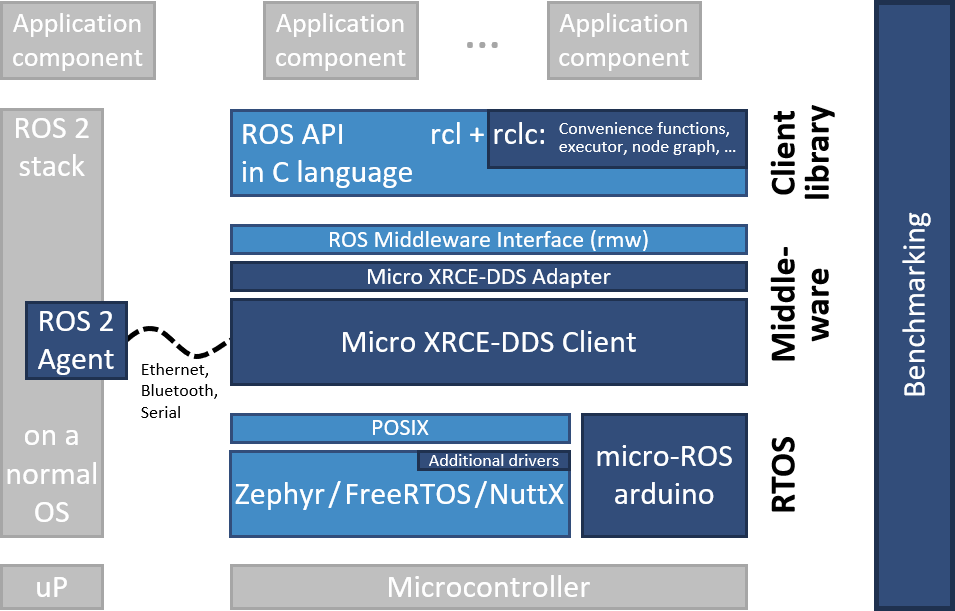
\includegraphics[width=0.8\textwidth]{imgs/Grundbegriffe/micro-ROS_architecture.png}
            \caption{Micro-ROS Architektur}
            \label{fig:micro-ros-architecture}%
        \end{figure}
    \end{description}
\end{flushleft}

\begin{flushleft}
    \textit{Technologischer Standpunkt Hardware:} \\
    Es existieren bereits viele Forschungen und Beispiele für diverse Roboter
    und deren verschiedensten Antriebskinematiken.
    Für unser Projekt werden wir allerdings eine eigene Roboter Platform designen und 3D-Drucken.
    Viele der bereits vorhandenen Roboter sind entweder zu Groß und teuer oder viel zu klein und deshalb ebenfalls nicht 
    gut für eine demonstration geeignet. Unter anderem wollen wir das unser Roboter den Vorteil bietet weitestgehend
    3D-gedruckt zu sein.
    Die ETH Zürich (TODO LINK?) hat bereits eine kleine Zusammenfassung über die wichtigsten Antriebsarten mobiler Roboter zur Verfügung gestellt.
    Für unser Projekt haben wir uns vorerst für einen simplen Diferentialantrieb entschieden. 
\end{flushleft}

\section{Lösungsideen}
\input{lösungsideen.tex}

\section{Evaluation der Lösungsideen anhand der Anforderungen}

\subsection{Evaluierung der Frontend-Frameworks/Bibliotheken}
\begin{flushleft}
    Da es unglaublich viele Web Frontend Frameworks gibt, die sich leider oft nur in minimalen Punkten unterscheiden,
    haben wir uns Schlussendlich für React aus den unten genannte Gründen entschieden.

    Da Ein Teammitglied bereits viel Erfahrung mit React sammeln konnte sahen wir das als starken Vorteil für unser Team an.
    Außerdem verfügt React über eine enorm gute Dokumentation, da es ständig von seiner eigenen Community verbessert wird.
\end{flushleft}

\subsection{Gründe für die Auswahl von ROS?}
\begin{flushleft}
    Da wir alle bereits mit ROS gearbeitet haben, ist die Softwareentwicklung für einen Microcontroller deutlich einfacher, da ROS viele Standard-Aufgaben wie die Interprozesskomunikation erledigt. Außerdem ist es für uns leichter bekannte Hürden zu umgehen.
    ROS stellt auch eine große Auswahl an Bibliotheken und Tools bereit, die die Entwicklung ebenfalls erleichtern und beschleunigen.\\
    
    Ein weiterer Grund dafür, dass wir uns für die Entwicklung mit ROS entschieden haben ist, dass wir im Robotiklabor viel Hilfe bekommen können, da dort alle Roboter mit ROS entwickelt werden.
    Weitere Vorteile von ROS sind, dass es open-source ist und kostenlos.

    
\end{flushleft}

\subsection{Micro-ROS und RTOS}
\begin{flushleft}
    Die Entwicklung mit dem Mikrocontroller findet mit Micro-ROS statt, da das die Standard-Bibliothek für die Entwicklung mit Microcontrollern mit ROS2 ist.\\
    Das Besondere an ROS2 und Micro-ROS im Vergleich zu ROS1 ist, dass es ermöglicht ein Real Time Operating System auf dem Microcontroller auszuführen. Ein RTOS wird standardmäßig mitinstalliert, ist aber für uns auch interessant, da wir bisher noch nicht mit RTOS gearbeitet haben und es eine gute Lernmöglichkeit mit beschränkten Aufwand ist.
    Wie ROS selbst, ist Micro-ROS open-source und kostenlos.\cite{ros} \cite{micro_ros}\\
    Außerdem gibt es eine bereits bestehende Toolchain namens ESP-IDF, die das Cross-Compilieren, Flashen, Monitoring und Debugging erleichtert.
    \cite{esp_idf}

\end{flushleft}

\subsection{Roboter Platform}
\begin{flushleft}
    Die Anforderungen an die Roboter Platform für dieses Projekt waren recht klein und einfach gehalten.
     
    Das wichtigste bei der Neuentwicklung und Design einer Roboter PLatofr
\end{flushleft}

%----Implementierung----
\section{Implementierung}

%FRONTEND
\subsection{React Front-End}

\subsubsection{Erstellung des Prototypes}
\begin{flushleft}

Der wichtigste Punkt war es nun eine lauffähige Schnittstelle zwischen ROS2 und einer Webanwendung herstellen zu können.
Für schnelles prototyping bietet die Open Source Robotic Foundation (OSRF) vorkonfigurierte Docker Container, in jeder beliebigen ROS Version, an.
Hierzu muss nur Docker Compose auf dem Rechner installiert sein, und ein fertiges Image kann sogleich erstellt werden.
%Um beispielsweise ein ROS2 Image mit der Foxy Fitzroy Version zu installieren, muss folgender Befehl ausgeführt werden. 
Für ein fertiges ROS Image mit der Foxy Fitzroy Version kann mit dem \textit{docker pull} [\ref{frontend_install}] Befehl installiert werden. 
% \begin{lstlisting}[language=bash]
%     docker pull osrf/ros:foxy-desktop 
% \end{lstlisting}

% \textit{foxy-desktop} kann hier mit jeder anderen beliebigen Version ausgetauscht werden. Mehr Informationen hierzu findet man im entsprechenden Docker Hub: 
% \begin{lstlisting}
%     https://hub.docker.com/r/osrf/ros/
% \end{lstlisting}

Da ROS Nodes über TCP/UDP Sockets kommunizieren, muss nun eine Brücke geschaffen werden, um Daten mit dem Web-Browser austauschen zu können.
Hier schafft das \cite[Rosbridge]{rosbridgepackage} Paket Abhilfe, in dem es einen Websocket erstellt, welcher in allen gängigen Web-Browsern unterstützt wird. Mit diesem Paket ist es nun möglich die bekannten Publish- und Subscribe-Funktionalitäten der ROS-Umgebung zu nutzen.
In der Abbildung \ref{fig:rosbridge_chain} wird die eben beschriebene Kommunikation vereinfacht dargestellt, sodass nun mehrere ROS Nodes mit dem Browser interagieren können.
\begin{figure}[h!]
    \centering
    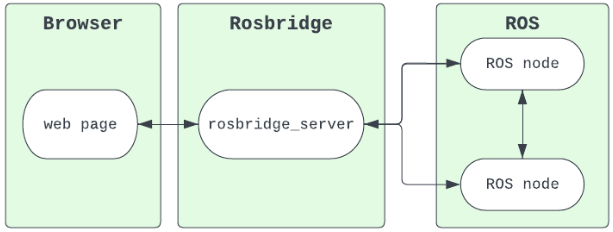
\includegraphics[width=0.8\textwidth]{imgs/web/rosbridge_chain.png}
    \caption{Rosbridge Kommunikation \cite{foxyglove_rosbridge_tut}}
    \label{fig:rosbridge_chain}%
\end{figure}
Die \textit{Rosbridge} kann ganz einfach über den apt-Paketmanager installiert werden.



% TODO Anhang Anleitung hinzufügen
Für eine genaue Anleitung um die \textit{Rosbridge} lauffähig zu bekommen, wird auf den Anhang verwiesen [\ref{frontend_install}].

Im nächsten Schritt wird eine einfache Webanwendung gebaut, die mit Hilfe der \textit{roslibjs} Bibliothek nun mit der \textit{Rosbridge} kommuniziert und Daten austauscht. 
Hierzu wird eine simple HTML-Seite erstellt und \textit{roslibjs} inkludiert. 

% \begin{lstlisting}[language=html]
% //Inkludierung und Quelle in HTML
% <script 
%     type="text/javascript" 
%     src="http://static.robotwebtools.org/roslibjs/current/roslib.min.js">
% </script> 


% \end{lstlisting}

% TODO Anhang Anleitung hinzufügen
Wenn nun die \textit{Rosbridge} erfolgreich in der ROS-Umgebung, in diesem Fall innerhalb des Docker Containers unseres Prototypens, gelauncht wurde, kann man sich mit einem Javascript-Objekt eine Verbindung zu dem Websocket aufbauen.
Hierzu wird die IP-Adresse des Docker-Containers mit dem Port 9090 benötigt.
Mit der URL \textit{ws://171.17.0.3:9090} haben wir uns beispielsweise in unserer Anwendung verbunden.
Ist die Verbindung erfolgreich hergestellt, können Publisher und Subscriber an das Objekt angebunden werden.
%Ausführliche Erklärungen und Code Beispiele sind im Anhang nachzulesen. (fehlt noch..)
Für eine 

Nachdem eine simple Schnittstelle zwischen ROS2 und einem Web-Browser erfolgreich hergestellt wurde, wird es im Folgenden um die Umsetzung der React-App gehen. 




\end{flushleft}

\subsubsection{Aufbau des Frontends (Architektur)}
\begin{flushleft}

Da zuvor noch keine Vorerfahrungen zum Erstellen von React-Apps bestand, erfolgte hier erst eine Einarbeitung in diverse Grundlagen und Funktionalitäten in  React.
React ist ein Javascript Framework zum Entwickeln von Webseiten und Webanwendungen.
Statt einfachen statischen HTML-Seiten wird hier mit sogenannten Komponenten gearbeitet, die mehrfach verwendet werden können.
Ebenso können mit States und Hooks reaktive Single-Page-Applications erstellt werden, die ein re-rendern der jeweiligen Komponenten erlauben, ohne ein Neuladen der ganzen Seite.
Weitere Pakete und Bibliotheken können mit dem Paketmanager npm ebenfalls jederzeit nachinstalliert werden.

So gibt es auch die \textit{roslibjs} Bibliothek im npm-Paketstore.
Installation und Importierung in das aktuelle Projekt wird in [\ref{frontend_install}] ausführlicher Beschrieben.
% \begin{lstlisting}[language=bash]
%     npm install roslib 
% \end{lstlisting}

% wird diese dem Projekt hinzugefügt und kann in folgender Weise inkludiert werden:

% \begin{lstlisting}
%     import ROSLIB from 'roslib';
% \end{lstlisting}

Bezüglich der Architektur, bzw. dem Aufbau der Website, haben wir uns an die standardmäßige Vorgehensweise in React gehalten, in dem man die Seite in Komponenten aufteilt und diese so an mehreren Stellen wieder verwenden kann. Dafür haben wir ein extra Verzeichnis \textit{/components} im \textit{/src} Verzeichnis angelegt, sowie eines mit \textit{/pages} für die jeweiligen Seiten. Diese werden in der \textit{App.js} Datei mit dem \textit{react-router-dom} Paket geroutet.


Wir haben uns für eine linksbündige Navigationsleiste entschieden, da diese mehr zu einem Dashboard und einer Konfigurationsseite passt. Auch hier wurde im ersten Moment nicht viel Wert auf ein besonders ausgefallenes Design gelegt. Eine schwarze Navigationsleiste mit einem aufklappbarem Burgermenü war hier für uns ausreichend. 

\hypertarget{rosboard-target}{Für} den generellen Aufbau und dem Design der Website hatten wir uns im Vorfeld schon Gedanken gemacht, so war es uns auf jeden Fall wichtig eine Übersichtseite mit allen Topics zu haben und von diesen die Inhalte auslesen zu können.
Im laufe der Wochen hatten wir ein Gespräch mit Benjamin Stähle aus dem RoboLab an der RWU, wir erzählten ihm von unserem Vorhaben und er zeigte uns ein ROS-Webdashboard namens \textit{rosboard}.
Diese Plattform hatte quasi die Funktionen, die wir für unsere Webanwendung auch geplant hatten.
Zu diesem Zeitpunkt überlegten wir uns, ob wir von nun an diese verwenden, oder unsere eigene Webanwendung programmierten.
Natürlich hätte es hier schon alle unsere gewünschten Funktionen zur Verfügung gehabt, allerdings entschieden wir uns dafür, einmal diesen Prozess von Grund auf selber zu entwickeln und unsere eigene ROS-Webanwendung zu erstellen.
Wir wollten uns aber vom Design und der Vorgehensweise trotzdem an der vorgestellten Anwendung von \textit{rosboard} orientieren.
Ebenso unterscheidet diese sich auch von der Implementierung, da diese auf ganz anderen Bibliotheken basiert.
\\

\vspace{0.5cm}
Um nun die Vorteile von React in unserer Anwendung sinnvoll zu nutzen, unterteilten wir das Connection-Handling, Publishen, Subscriben oder auch beispielsweise die Auflistung der aktuellen Topics, in eigene Komponenten auf.
So konnten wir mit Hilfe von useState-Hooks und useContext-Hooks, eine Singlepage-Application bauen, die mehrere Verbindungen zu ROS-Instanzen verwalten kann.
Für jede offene Verbindung wird ein neues ROSLIB-Objekt angelegt und in ein Array gespeichert.
So kann für jedes dieser Objekte eine neue eigene Unterseite erstellt werden, um mit den ROS-Topics zu interagieren. Diese werden ebenso im Dashboard in einer Tabelle ausgegeben (siehe Abbildung \ref{fig:ros_conn}).

\begin{figure}[h!]
    \centering
    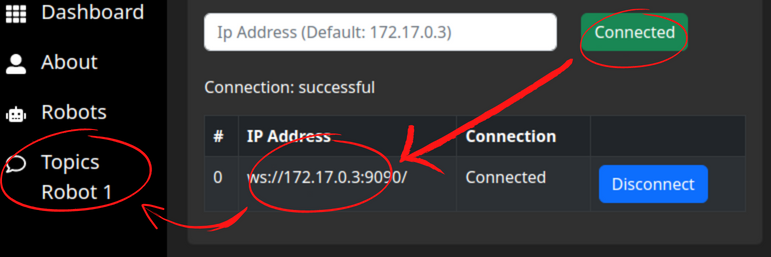
\includegraphics[width=0.8\textwidth]{imgs/web/ros_conn.png}
    \caption{Connection Handler mit Liste und automatischem Navigationspunkt}
    \label{fig:ros_conn}%
\end{figure}

Auf diesen nun generierten Topics-Unterseiten des jeweiligen Roboters, können nun Funktionen darauf angewendet werden.
Für das Publishen auf Topics haben wir uns nur auf das \textit{/cmd\_vel} Topic beschränkt, was einen recht simplem Grund hatte.
Denn zum Publishen wird natürlich auch der Message-Type der Nachricht benötigt.
Um dann dynamisch auf jedes beliebige Topic senden zu können, müsste der User ebenso, auch den entsprechenden Aufbau der Nachricht haben und diese richtig in ein Textfeld eingeben.
Dies wäre sowohl aus User Sicht sehr umständlich und fehleranfällig, da die einzelnen Werte nicht mehr in simplen vordefinierten Textfeldern, sondern in freien Textareas, hätten abgefragt werden müssen. 
Da das \textit{/cmd\_vel} Topic, welches für die Fortbewegung und Lenkung des Roboters zuständig ist, unser definitiv wichtigstes Topic war, beließen wir es dabei.
Dieser Nachrichtentyp enthält drei linear- und drei angular-Werte:

\label{sec:twistMessage}
\begin{lstlisting}
    twist = {
        linear: {
            x: 0,
            y: 0,
            z: 0
        },
        angular: {
            x: 0,
            y: 0,
            z: 0
        }
    }
\end{lstlisting}
Wobei für die Fortbewegung bei Robotern, die sich auf dem Boden mit Rädern bewegen, nur die x-Werte in \textit{linear} und \textit{angular} interessant sind.
Hierfür haben wir im Frontend zwei Optionen entwickelt. 
Zum einen war es uns wichtig fest definierte Werte senden zu können, wofür wir uns für einzelne Textfelder pro Wert entschieden.
Diese wurden dann im Code auf das entsprechende Message Format (Twist) gebracht und an die \textit{rosbridge} gesendet.
Links in Abbildung \ref{fig:web_publish} sind die Textfelder, mit den jeweiligen Buttons zum Senden und Rücksetzen der Nachricht.
Bei Reset wird einfach eine neue Nachricht geschickt, die alle Werte wieder auf Null setzt.

\begin{figure}[h!]
    \centering
    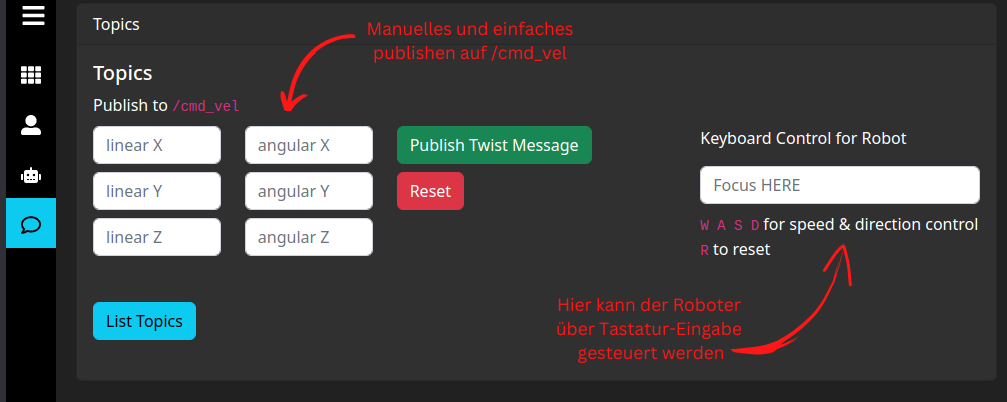
\includegraphics[width=0.8\textwidth]{imgs/web/web_publish.png}
    \caption{Zwei Möglichkeiten um auf \textit{/cmd\_vel} zu publishen}
    \label{fig:web_publish}%
\end{figure}

Ebenso dachten wir uns auch, dass es eine gute Funktionalität wäre, wenn man den Roboter über Tastatur-Eingabe steuern könnte.
So erstellten wir noch ein Textfeld, welches beim Fokussieren die Tastenfelder einließt.
Dies konnte mit dem Event-Handler \textit{onKeyPress} in React umgesetzt werden.
Durch Gedrückthalten der Tasten W, A, S, D, wird der entsprechende linear- oder angular- x-Wert inkrementiert, bzw. dekrementiert.
Mit der Taste R wird auch diese Nachricht wieder zurückgesetzt.
In Abbildung \ref{fig:web_publish} ist dies auf der rechten Seite zu sehen.
Im Anhang in [\ref{webroscomm_code}] wird einmal kurz der Vorgang des Publishen und Subscribens an einem Codebeispiel gezeigt.
\\

\vspace{0.5cm}
Als letztes soll noch auf das Subscriben zu offenen Topics über die Webanwendung beschrieben werden.
Über den Button "List Topics", werden alle momentan zur Verfügung stehenden Topics angeordnet. 
Wie in Abbildung \ref{fig:web_subscribe} zu sehen ist, öffnet sich unterhalt der Topic-Liste ein Fenster für das jeweilige Topics. 
Bei mehreren werden diese nebenbei oder darunter automatisch aufgelistet. 
Innerhalb des Festers werden alle neu ankommenden Nachrichten im JSON-Format gelistet.

\begin{figure}[h!]
    \centering
    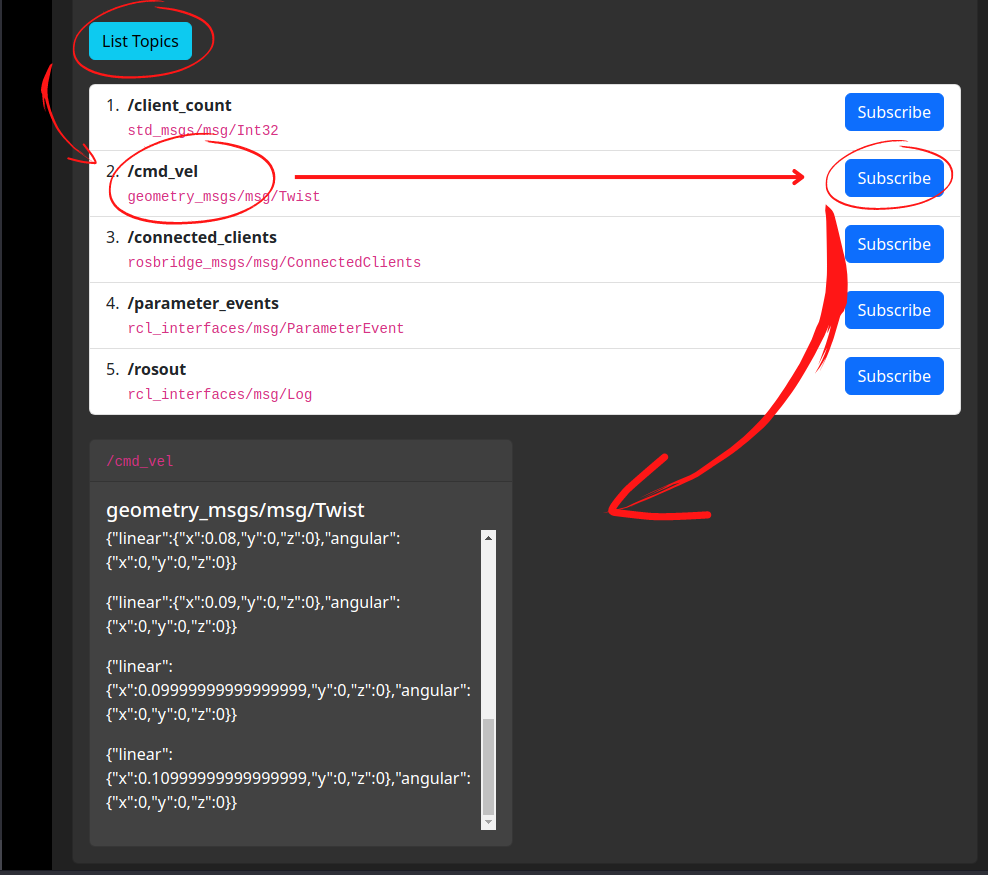
\includegraphics[width=0.8\textwidth]{imgs/web/web_subscribe.png}
    \caption{Topics Liste und Subscription zu \textit{/cmd\_vel} Topic}
    \label{fig:web_subscribe}%
\end{figure}

\end{flushleft}
    


%BACKEND
\subsection{ROS Back-End}
\subsubsection{Firmware Kompilierungs Toolchain}
\begin{flushleft}


    Um Programme auf dem ESP32 ausführen zu können müssen sie zuvor crosscompiled und auf den Speicher des Mikrocontrollers geflasht werden.
    Für das Crosscompilen von Programmen, die das Micro-ROS Framework verwenden wird eine Pipeline empfohlen, die aus 4 Teilen besteht.
    \begin{enumerate}
        \item ROS
        \item Micro-ROS
        \item RTOS
        \item ESP-IDF
    \end{enumerate}

    Zu Grunde liegt ersteinmal die ROS2 Compilierungspipeline welche colcon verwendet.
    Darauf aufbauend folgt die Micro-ROS Pipeline. In dieser Pipeline wird die Crosscompilierung für das entsprechende Realtime Operating System übernommen.
    Des weiteren wird noch die ESP-IDF Pipeline verwendet, die für die Crosscompilierung für den ESP32 zuständig ist und mit deren Hilfe die Programme auf den Mikrocontroller geflasht werden können \cite{esp_idf}.

    Die Pipeline welche gerade beschrieben wurde, wurde mit Hilfe von Docker implementiert \cite{docker_best_practices}.

    Als erstes wird ein neuer User inklusive Home-Verzeichnis und entsprechenden Cgroup Berechtigungen angelegt.
    Für die Berechtigungen ist vor allem die dialout-Gruppe wichtig, da diese Zugriff auf seriellen Ports gibt.

    Die Verwendung eines eigenen Users ohne root-Rechte wird verwendet, 
    da es von Docker als Best-Practice empfohlen wird um ungewollte Veränderungen zu verhindern.


    Nach dem Aufsetzen des Users wird die Micro-ROS Pipeline heruntergeladen und mit Hilfe von mitgelieferten Skripten installiert.

    Nach der Installation müssen noch verschiedene Einstellungen vorgenommen werden. So ist es in eine ersten Schritt notwendig das passende RTOS, in diesem Fall \textit{freertos},
    und den Mikrocontroller zu spezifizieren \cite{freertos}. Anschließend werden Einstellungen wie beispielsweise die Zugangsdaten für das WLAN-Netzwerk eingetragen.

    Es ist außerdem noch notwendig den host-user zu den cgroups docker und dialout hinzuzufügen, 
    da es ansonsten nicht möglich ist den Container zu starten oder Programme auf den Mikrocontroller zu übertragen.


    Für das erleichterte Ausführen des Containers wird eine docker-compose-Datei verwendet.

    Der Container wird mit zwei bind-mounts eingerichtet. Einer für das Verzeichnis, 
    in dem der Code des Roboters ist und ein anderer für das Verzeichnis \textit{/dev} in dem die Ports für das flashen des Mikrocontrollers sind.

    Es werden bind-mounts verwendet, um die Daten und Ports während der Entwicklung aktuell zu halten, damit der Container nicht ständig neu gestartet werden muss, wenn sich eine Datei ändert.
    Das vereinfacht die Entwicklung deutlich, da der Container beim An- und Abstecken des Mikrocontrollers nicht neu gestartet werden muss. 
    
\end{flushleft}


%HARDWARE
\pagebreak
\subsection{Roboter Platform}
\subsubsection{3D-Druckteile}
\begin{flushleft}
    Die Wichtigste Anforderung an die Platform war, dass diese Modular aufgebaut werden kann. Denn dann ist es möglich, auch im Nachhinein
    neue Teile, Module oder komplett andere Sensoren einfach anzuschrauben, bzw. auch kaputte oder alte Teile problemlos zu erneuern.

    Da es sich beim Differentialantrieb nur um eine mechanische Anordnung der Motoren selbst handelt, musste noch ein
    geeignetes Bauteil als Motor selbst gefunden werden.
    Die Motoren müssen ein recht hohes Drehmoment, aber eine kleine Umdrehungszahl pro Minute aufweisen.
    Initial war es deshalb die Idee für normale 5V Motoren, wie sie auch in DVD Laufwerken verwendet werden, ein kleines
    Getriebe zu konzeptionieren und zu bauen, wie es in Abbildung \ref{fig:prototyp_transmission} zu sehen ist.

    \begin{figure}[h!]
        \centering
        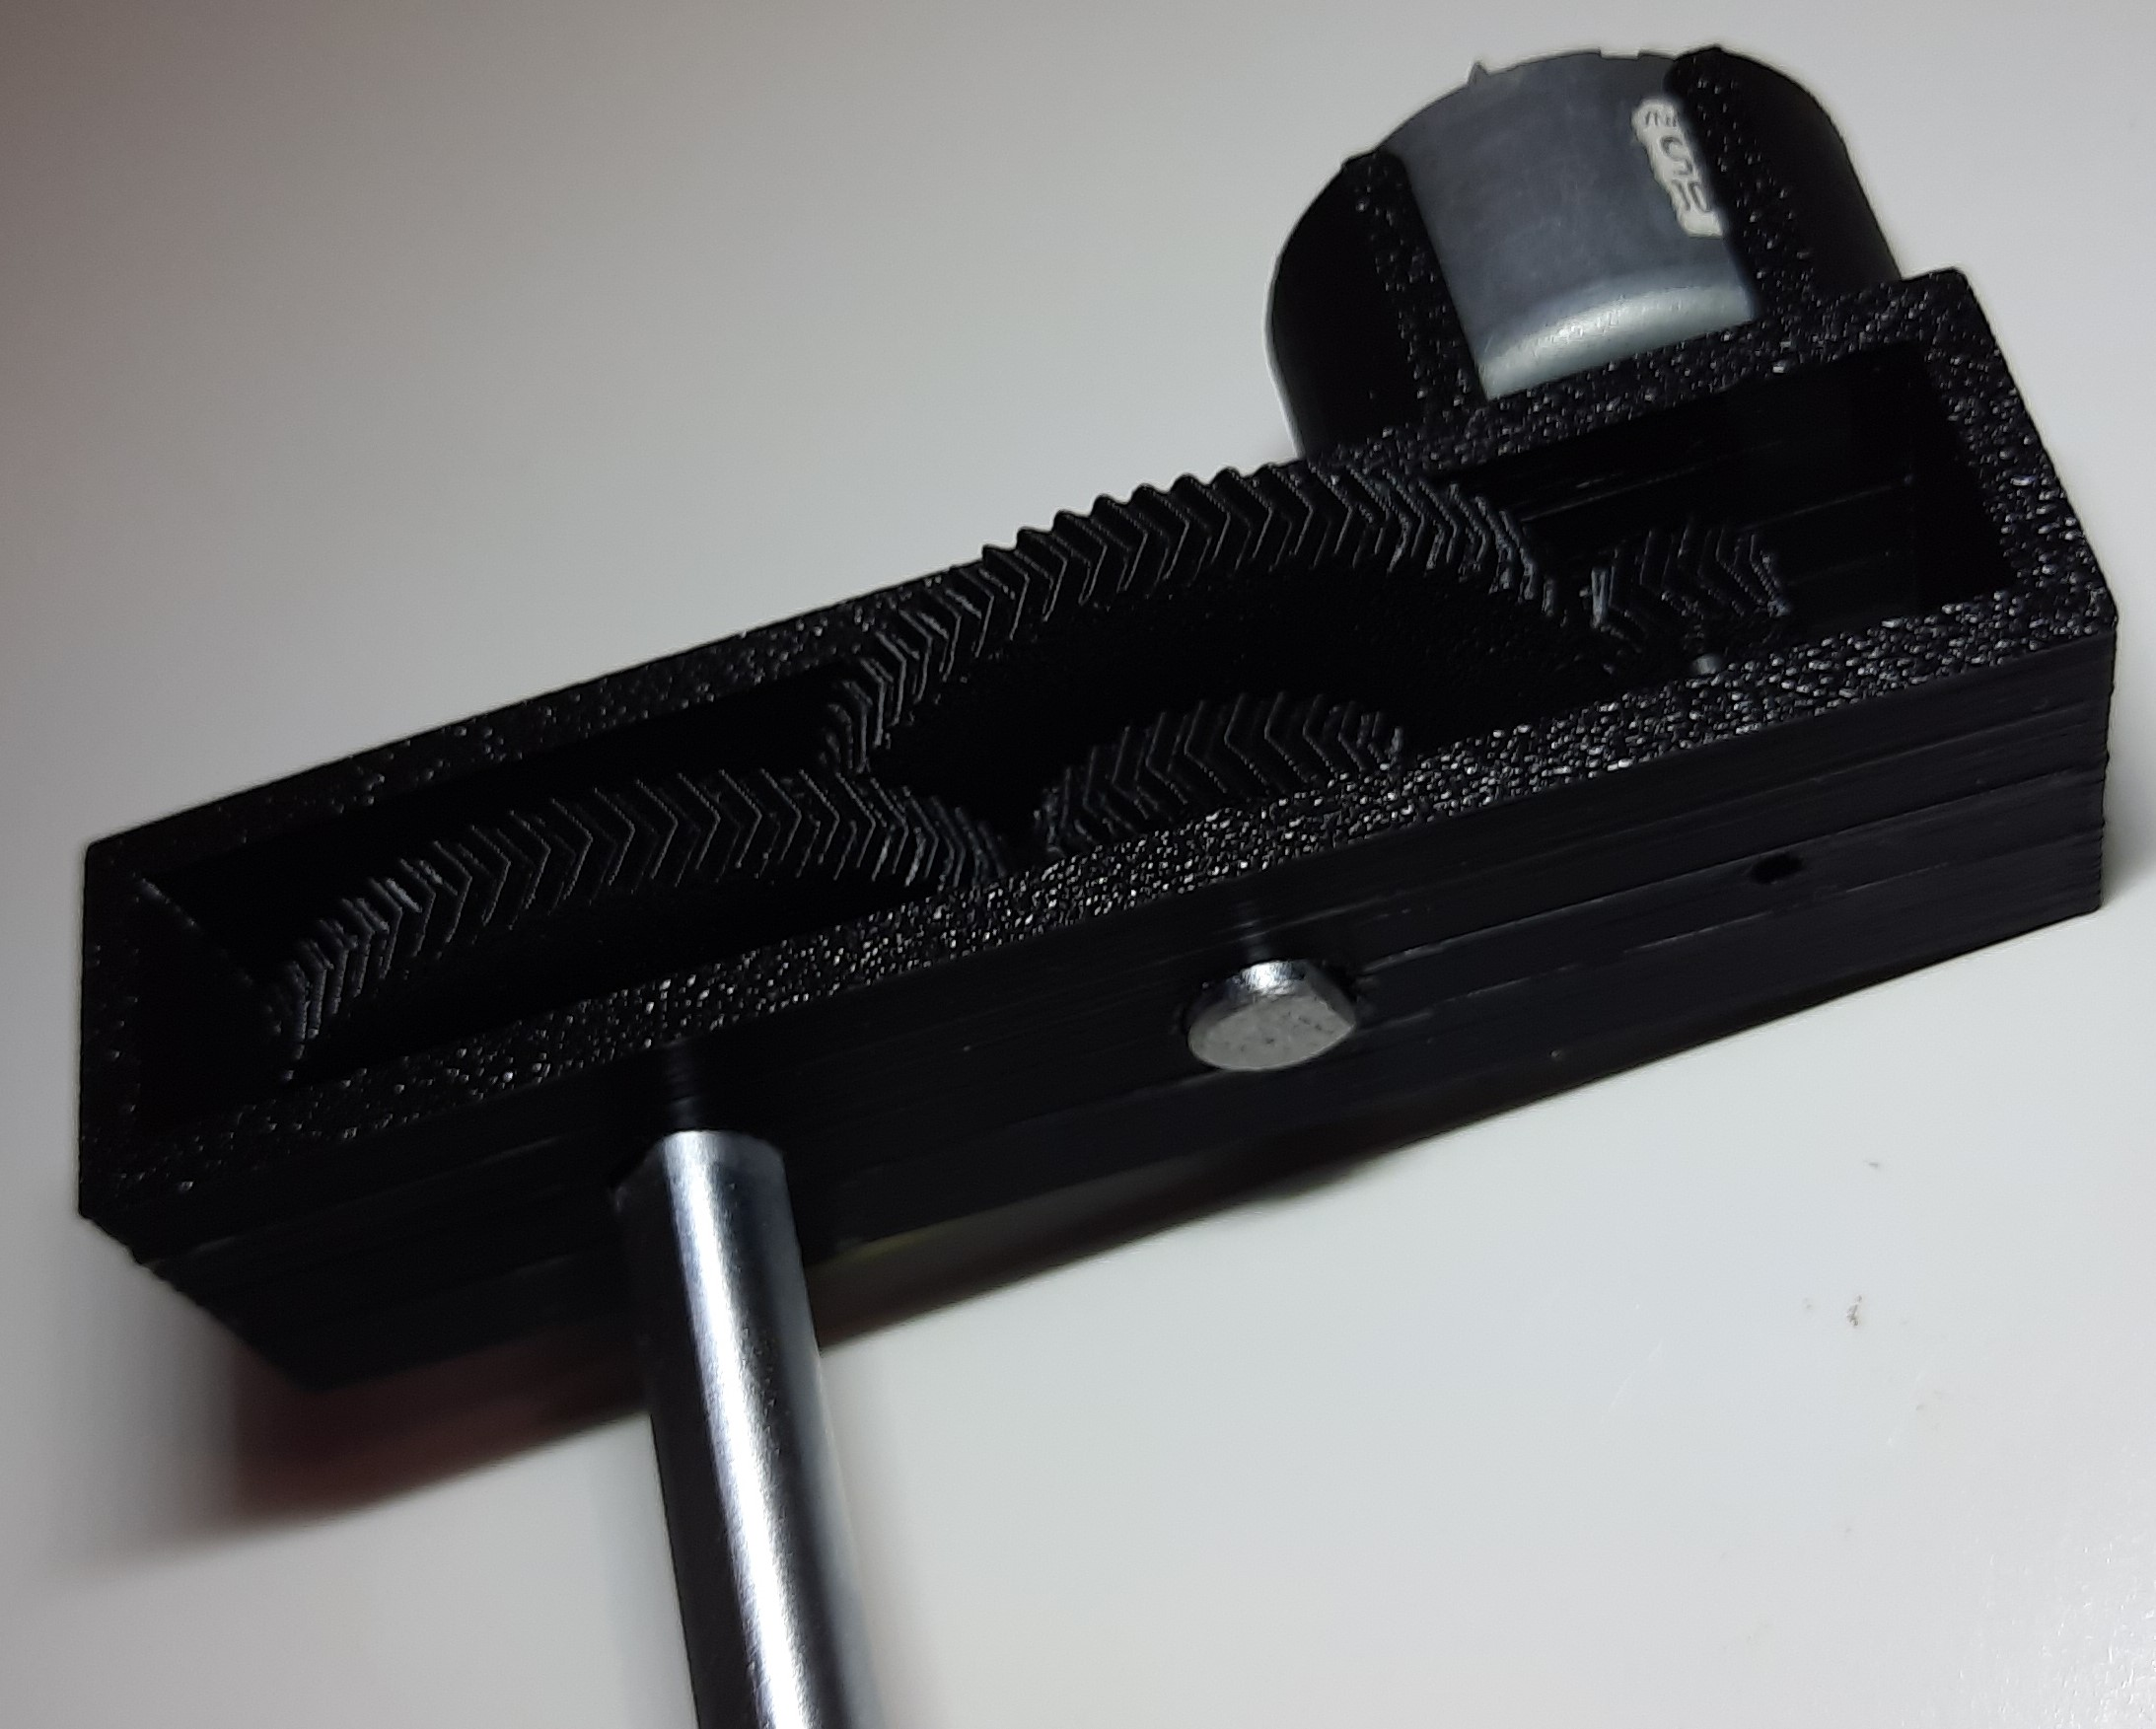
\includegraphics[width=0.3\textwidth]{imgs/Roboter/Real/Getriebe.jpg}
        \caption{Prototyp Eigenbau-Motorgetriebe}
        \label{fig:prototyp_transmission}%
    \end{figure}

    Die Idee bewies sich aber recht schnell als zu schwierig und wurde deshalb fallen gelassen.
    Als Ersatz für unseren misslungenen Versuch fiel die Entscheidung auf den Modellbau von Getriebemotoren (siehe Abbildung \ref{fig:robot_motor}).

    \begin{figure}[h!]
        \centering
        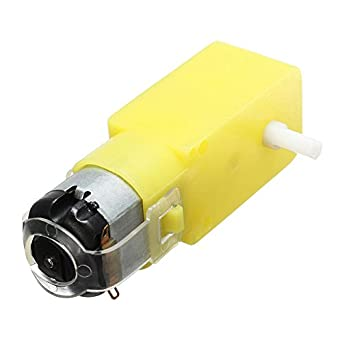
\includegraphics[width=0.3\textwidth]{imgs/Roboter/Real/41eJJZ8mOOL._SX342_.jpg}
        \caption{Modelbau Getriebemotor}
        \label{fig:robot_motor}%
    \end{figure}

    Ein Anforderung an unsere Demo Roboter Platform war die 3D-Druckbarkeit, sowie deren Modularer Aufbau.
    Das Fahrgestell unseres Roboters setzt sich aus insgesamt 3 Modulen zusammen.
    Die Motorenhalterung woran die Motoren selbst und auch die H-Brücke befestigt sind.
    Die Zentrale Platform für unseren Mikrocontroller.
    Und die beiden Freirollen an der Front des Roboters.

    Die gesamte Roboter Platform wurde mit Hilfe eines iterativen Design-Prozesses gestaltet. 
    Zu Begin wurde nur das Fahrgestell des Roboters designed und gedruckt (siehe Abbildung \ref{fig:cad_fahrgestell}).

    \begin{figure}[h!]
        \centering
        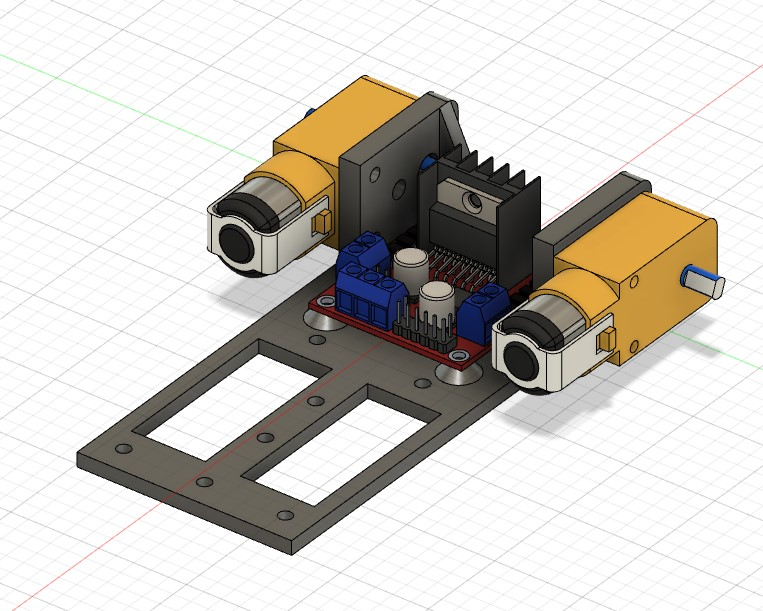
\includegraphics[width=0.3\textwidth]{imgs/Roboter/CAD/Fahrgestell.jpg}
        \caption{CAD Render vom finalen Fahrgestell}
        \label{fig:cad_fahrgestell}%
    \end{figure}

    Sobald das Ergebnis zufriedenstellend war wurde das nächste Modul designed und gedruckt.
    Dadurch erreichten wir eine Art Designkette und konnten sicherstellen das alle Teile bzw. Module zusammen passen
    und allen Anforderungen gerecht werden.
    Die letzten beiden Module für unseren Demo Roboter waren die Platform für die Elektronik (Abbildung \ref{fig:example} links) sowie die Freilaufrollen (Abbildung \ref{fig:example} rechts)
    an der Front des Roboters.

    \begin{figure}[h!]
        \centering
        \subfloat[\centering Elektronik Platform (finales Design)]{{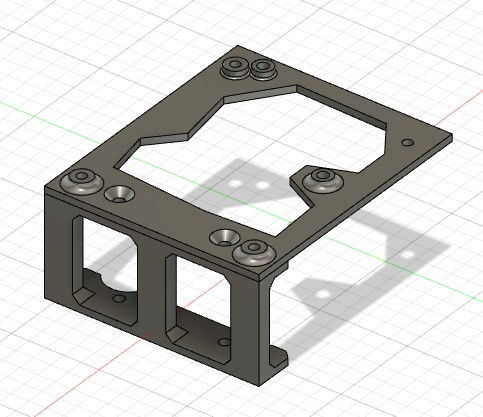
\includegraphics[width=0.3\textwidth]{imgs/Roboter/CAD/platform.jpg} }}%
        \qquad
        \subfloat[\centering Freilaufrollen (2. Version)]{{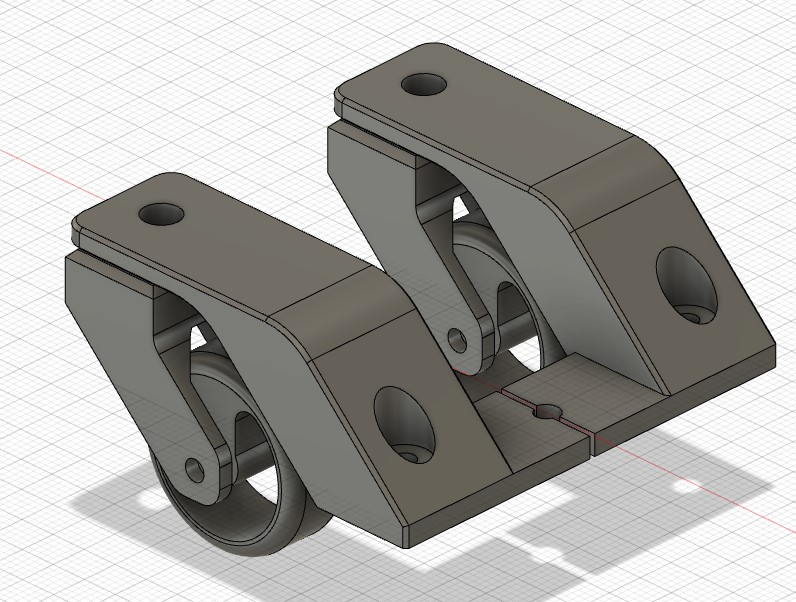
\includegraphics[width=0.3\textwidth]{imgs/Roboter/CAD/follower wheel.jpg} }}%
        \caption{CAD Render der Elektronik Platform und den Freilaufrollen}%
        \label{fig:example}%
    \end{figure}
\end{flushleft}

\subsubsection{Elektronik}
\begin{flushleft}
    Wie in unserer Evaluation der Lösungsideen bereits beschrieben übernimmt der ESP32 Microcontroller, siehe Abbildung \ref{fig:esp32_mc}, die Steuerung unseres Roboters. 
    
    \begin{figure}[h!]
        \centering
        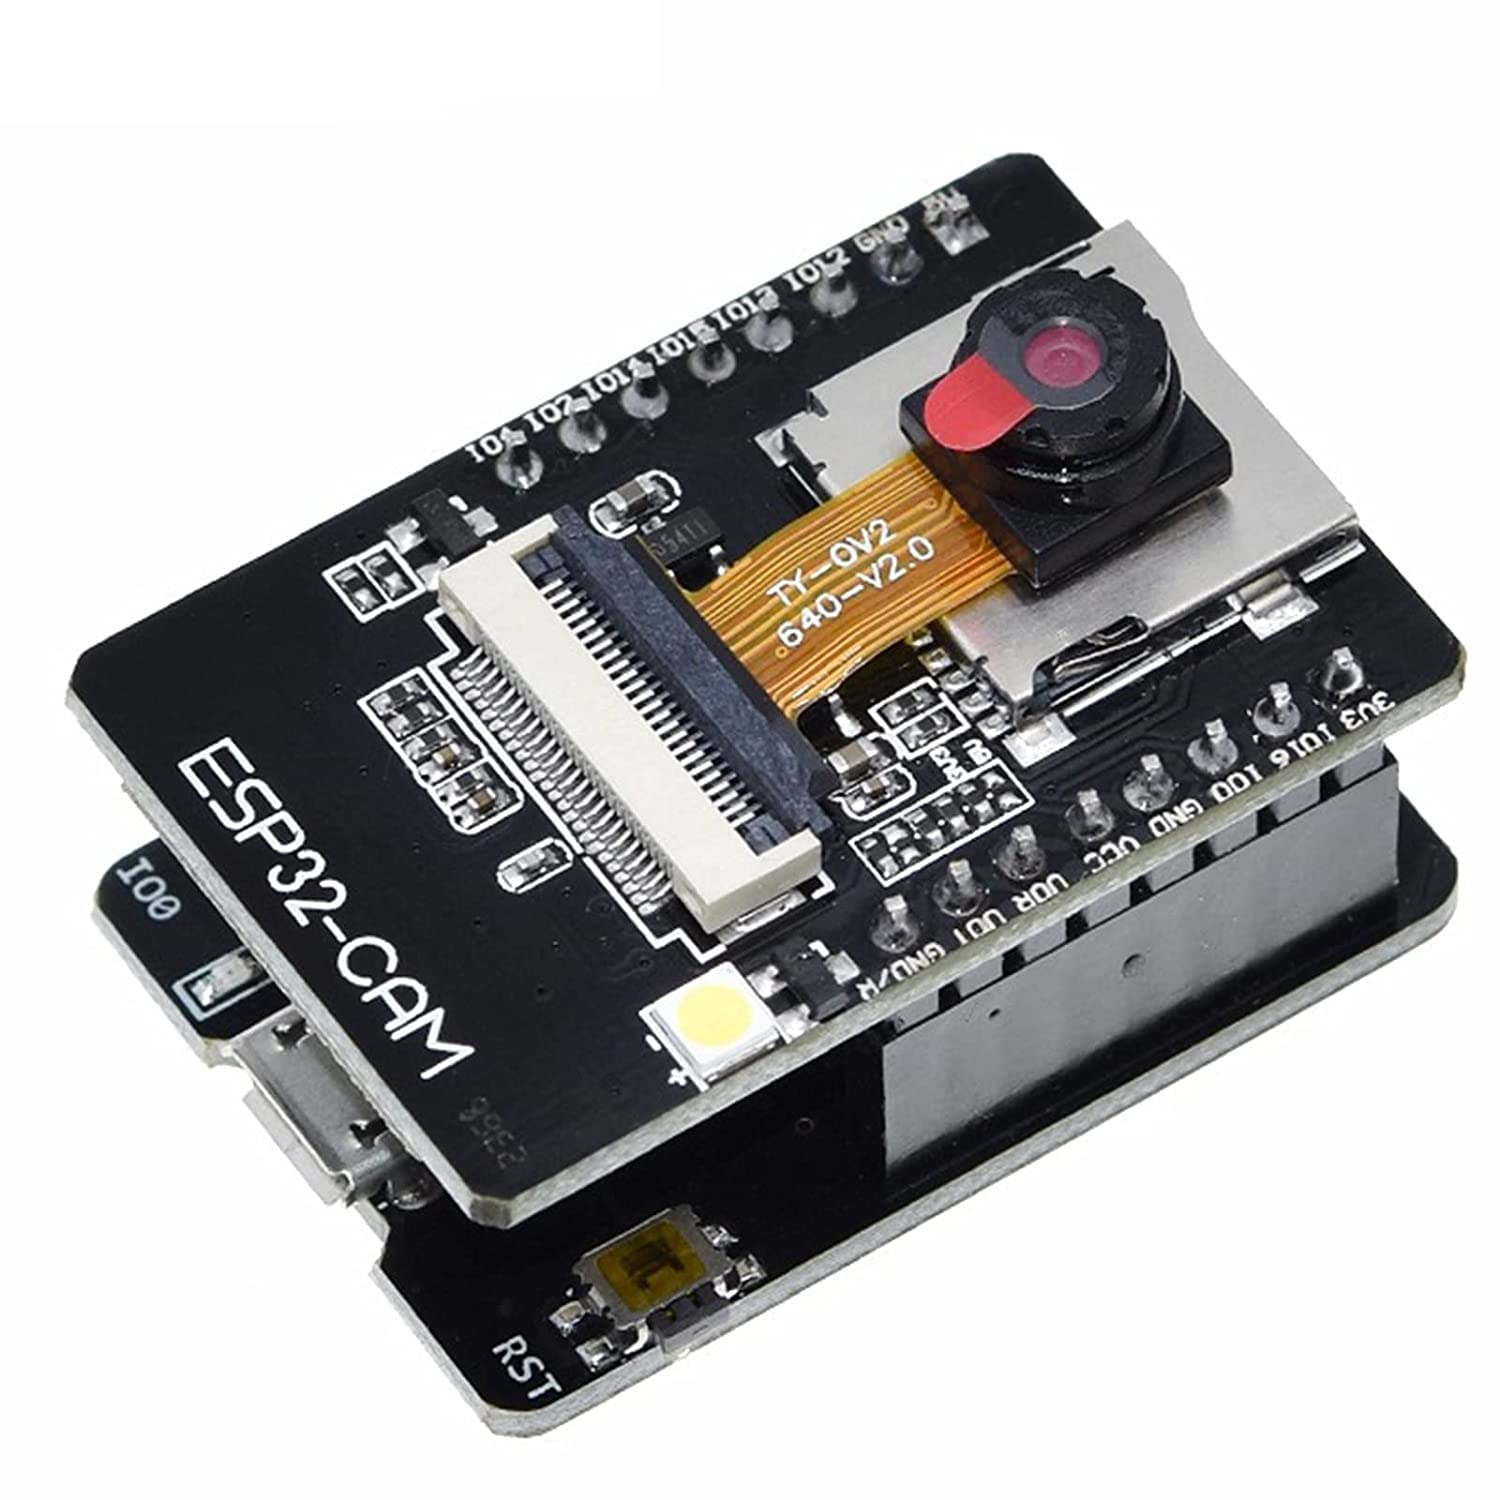
\includegraphics[width=0.3\textwidth]{imgs/Roboter/Real/esp32.jpg}
        \caption{ESP32 Microcontroller}
        \label{fig:esp32_mc}%
    \end{figure}

    Dieser muss natürlich auch mit Spannung versogt werden.
    Der Akku unseres Roboter sind sogenannte 18650 LiIon Akkus, diese sind wiederaufladbar und haben die perfekte Größe 
    für unseren kleinen Roboter.

    Die Versorgungsspannung für die Motoren kann direkt von unserem Akkupack abgegriffen werden und zur H-Brücke geführt werden.
    Die H-Brücke benötigt genau so wie der ESP32 eine Versorgungsspannung für die Logik.
    Diese sollte laut Datenblatt bei 5V liegen, erlaubt sind aber auch 3V. Was in unserem Fall ideal ist da unser ESP32
    ebenfalls nur mit 3,3V maxmimal versorgt werden darf.

    Die 3,3V Logikspannung werden auf unserer Platine von einem LM317T, einem Lineareren Spannungswandler zur Verfügung gestellt.

    \begin{figure}[h!]
        \centering
        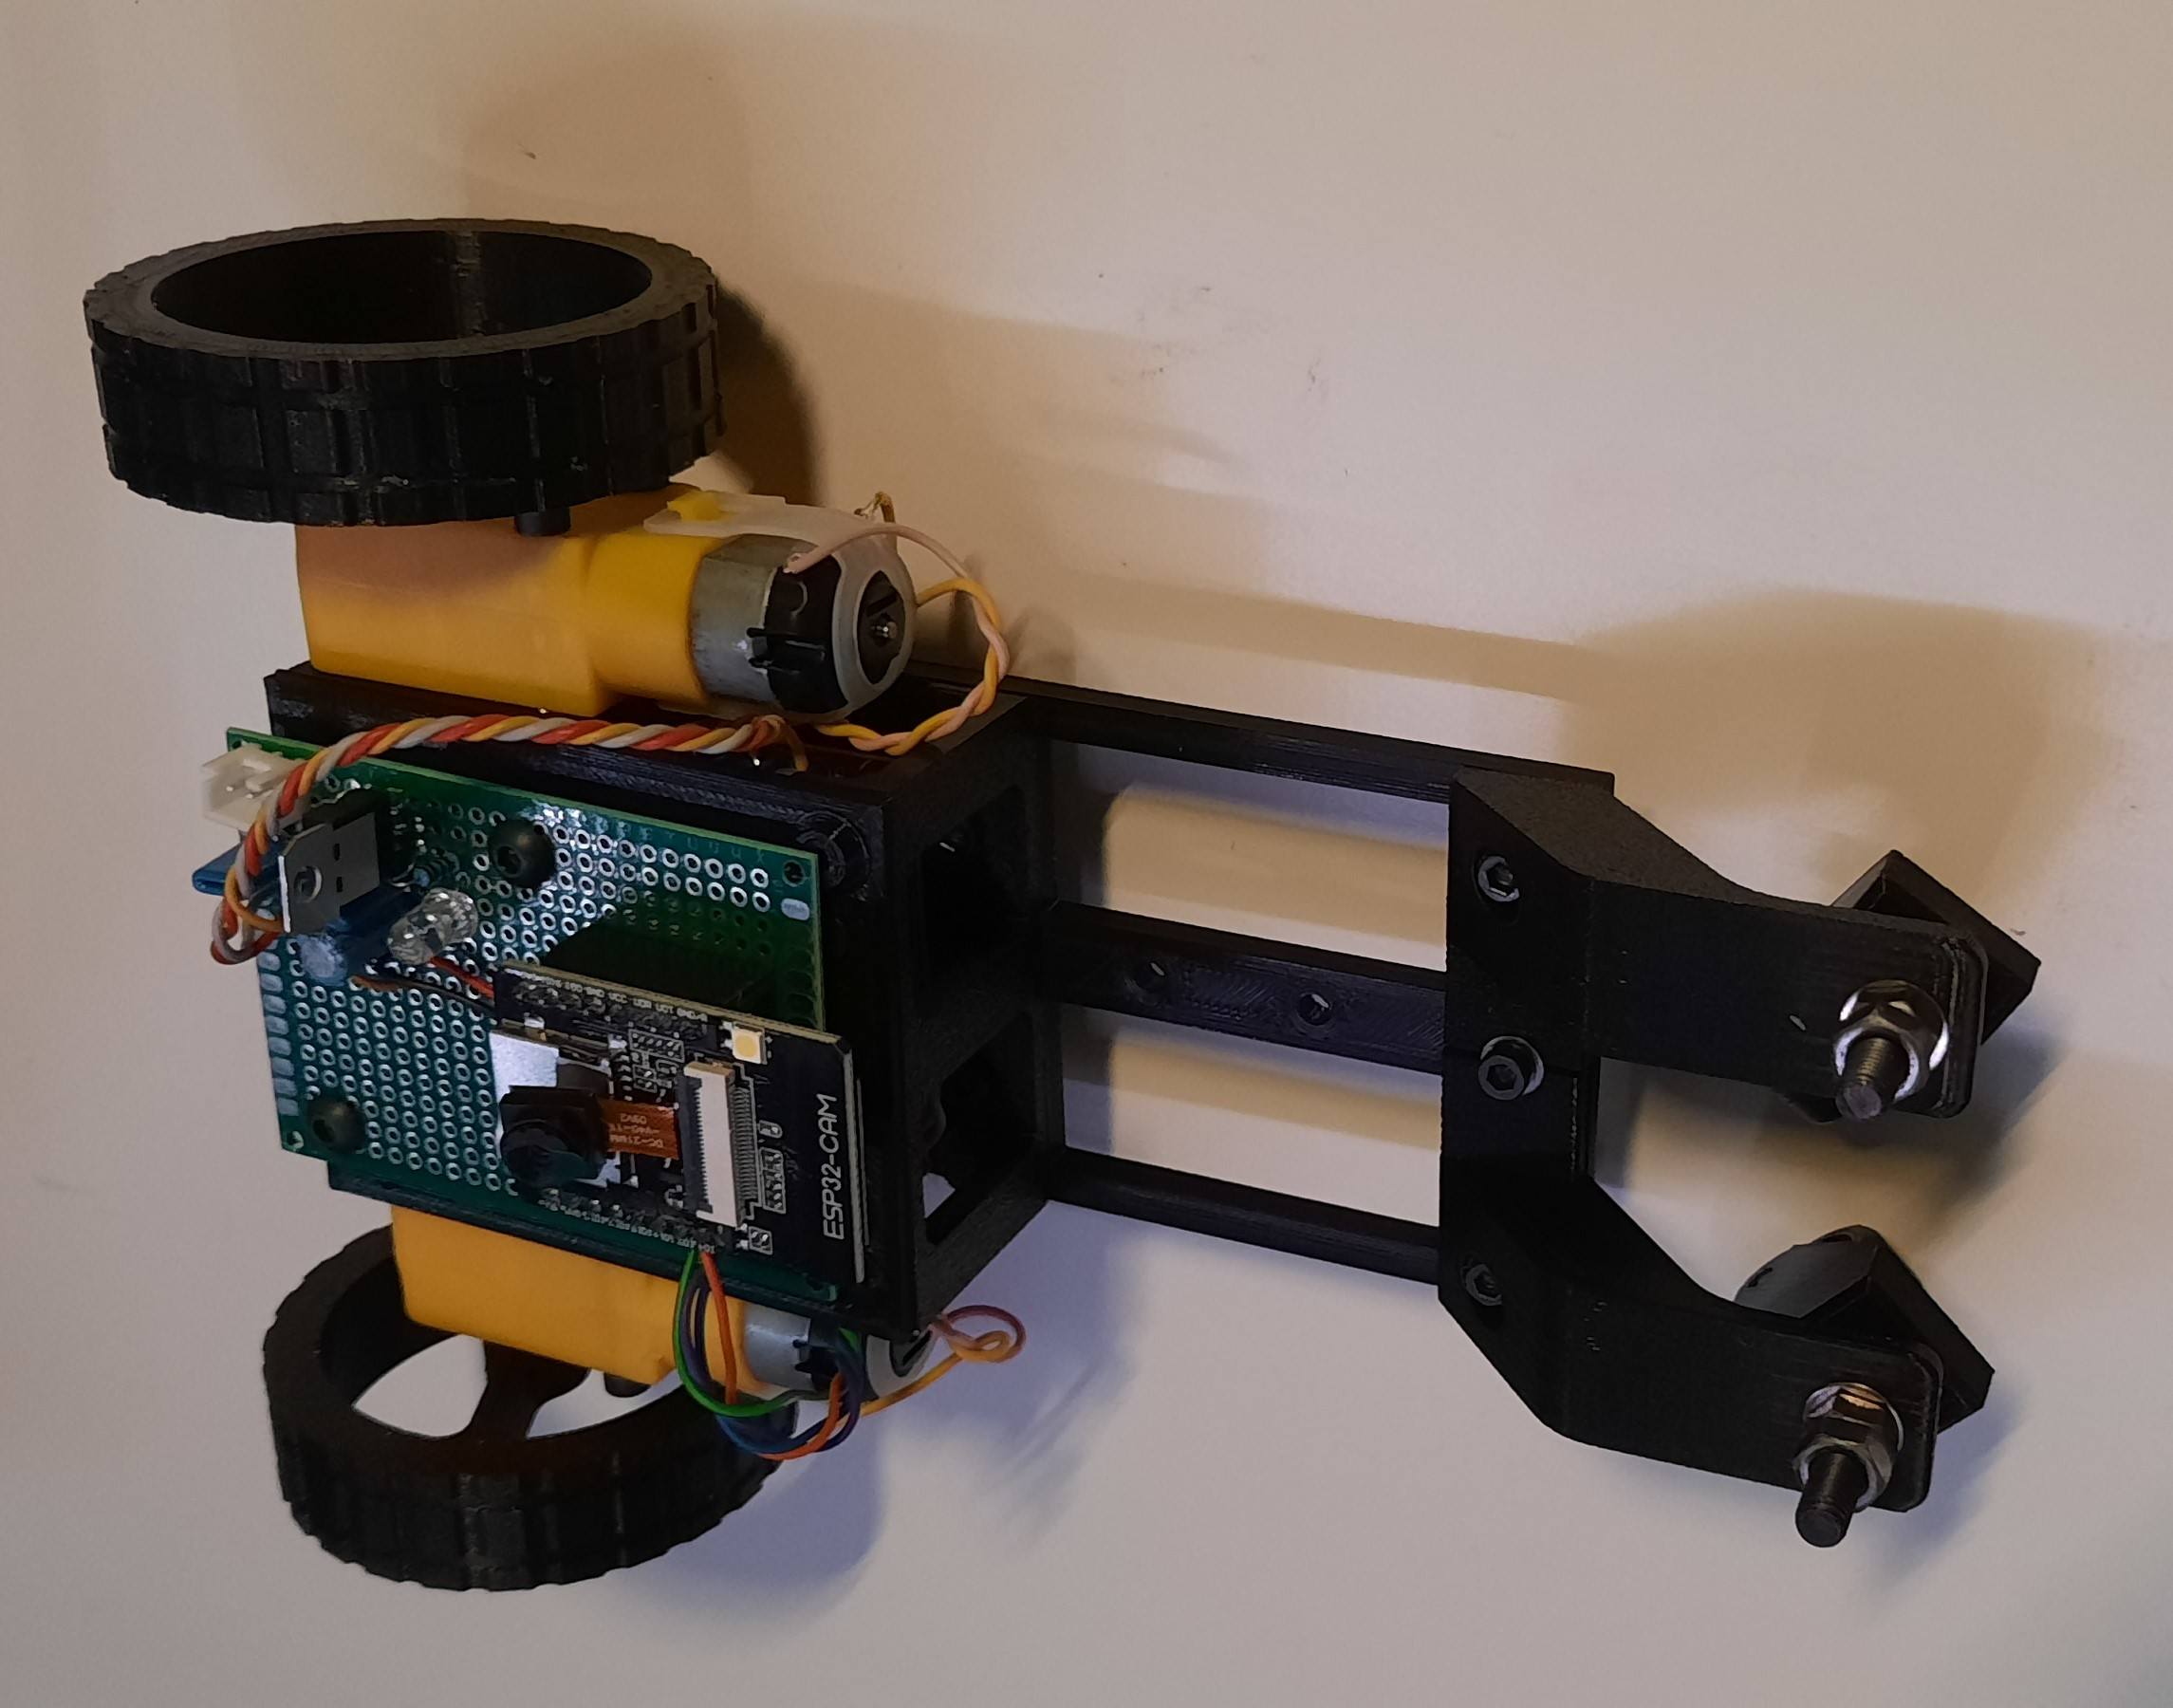
\includegraphics[width=0.5\textwidth, angle=-90,origin=c]{imgs/Roboter/Real/Roboter.jpg}
        \caption{Roboter Demo Platform}
      \end{figure}

\end{flushleft}

\section{Evaluation der Implementierung}

\subsection{Fehler und Verbesserungen Frontend}
\begin{flushleft}
    Am Anfang des Projektes planten wir neben dem Publishen und Subscriben der Topics, sowie einer Auflistung der aktuell offenen Topics, noch eine interaktive Konsole.
    Dies umzusetzen stellte sich aber schwieriger als gedacht heraus. 
    Es gab zwar gewisse Tools wie \textit{Xterm.js}, die so etwas ermöglichen sollten, was aber vor allem in Verbindung mit React nicht zum laufen gebracht werden konnte.
    Auch gäbe es einige Node.js Funktionalitäten, um Terminal-Befehle ausführen zu können, doch auch diese stehen unter der Verwendung von React nicht zur Verfügung, da es sich hier um eine isolierte Umgebung handelt und somit ein Zugriff auf OS System Prozesse nicht möglich ist.

    Aus diesem Grund beschlossen wir die interaktive Konsole in der Webanwendung zu streichen.

    Des weiteren hätten wir noch viele spannende Ideen für unsere Webanwendung gehabt.
    Beispielsweise das Speichern von Konfigurations-Einstellungen für einen Roboter.
    Hier wäre auch eine Datenbankanbindung denkbar.
    Ebenso das Publishen auf beliebige Topics, dessen Nachrichten-Typ der Benutzer nicht kennt.
    Sowie das Publishen auf benutzerdefinierte Topics, die in der Webanwendung ebenfalls angelegt hätten angelegt werden können.
    
    Allerdings hat uns dafür deutlich die Zeit für gefehlt, da allein das Einlernen in React anfangs schon viel Zeit in Anspruch genommen hat.
\end{flushleft}

\subsection{Fehler und Verbesserungen Backend}
\begin{flushleft}
    Beim Aufsetzen der Pipeline ist es mehrfach zu Problemen gekommen, die es notwendig gemacht haben, die Implementierung anzupassen.

    Zu Beginn wurde erst einmal mit Hilfe einer virtuellen Maschine ausprobiert, ob die Micro-ROS-Pipeline überhaupt funktioniert mit dem ESP32.
    Das hat gut funktioniert, es hat sich aber herausgestellt, dass die Pipeline sehr viel Speicherplatz benötigt und sie relativ tief ins System eingreift.
    
    Als nächstes sollte dann die Pipeline mittels Docker umgesetzt werden, um zum einen die Verwendung einer virtuellen Maschine zu vermeiden, aber trotzdem die Virtualisierung beizubehalten.

    Für die Virtualisierung mit Micro-ROS mit Docker gab es 3 Möglichkeiten:
    \begin{enumerate}
        \item Die Verwendung der ESP-IDF Toolchain als Extension für VSCode.
        \item Die Verwendung von micro-Ros docker Extension
        \item Die Erstellung eines eigenen Docker-Images
    \end{enumerate}

    Zuerst wurde die ESP-IDF Pipeline mit Hilfe einer Anleitung aufgesetzt. 
    Während dem Aufsetzen ist es zu einem Problem mit Docker-Desktop gekommen. Die ESP-IDF-Extension mit Docker funktionieren, allerdings funktioniert sie nur mit dem standard-Context von Docker, der aber von Docker-Desktop verändert wird.
    Somit war es notwendig Docker-Desktop wieder zu entfernen und zu Docker-Engine zu wechseln.

    Mit Docker-Engine war es dann möglich die ESP-IDF-Extension mit VSCode auszuführen und Code auf den ESP32 zu flashen.
    Die ESP-IDF Extension hat aber den Nachteil, dass es für uns notwendig wird, die ganze restliche Micro-ROS Pipeline selbst aufzusetzen.

    Also wurde als nächstes die Micro-Ros docker Extension für ESP-IDF ausprobiert. Diese stellt die ein Docker-Image zur Verfügung, das in die ESP-IDF integriert werden kann. Das behebt das Problem, des händischen Aufsetzens der Pipeline wie im vorherigen Schritt.
    Hierbei wurde einmal versucht den debugger zu testen. Grundsätzlich ist der openOCD Server, der Debugging ermöglicht hochgefahren. Allerdings war es danach nicht mehr möglich mit der ESP-IDF-Extension aus dem ersten Schritt auszuführen. 
    Anscheinend hatte die Ausführung dieses OpenOCD-Servers Einstellungen in der Konfiguration von VS-Code docker gemacht, die zur Folge hatten, dass die ESP-IDF-Extension nicht mehr richtig ausgeführt werden kann.

    Da sich herausgestellt hat, dass die ersten beiden Methoden nicht zuverlässig waren, wurde schließlich die letzte Methode gewählt: Wir haben ein eigenes Docker Image erstellt.
\end{flushleft}

\subsection{Fehler und Verbesserungen Roboter Platform}
\begin{flushleft}
    Getriebe selber bauen sollte doch kein Problem sein, oder?:
    Initial sollten kleine 5V Motoren aus alten DVD-Laufwerken mit selbstgebauten getriebe als Antrieb dienen.
    Jedoch musste man recht schnell festellen dass das Design von einem Getriebe doch nicht so einfach ist.
    Es muss auf den perfekten Abstand der Zähne der Zahnräder geachtet werden. Das die Zahnräder konzentrisch und 
    sich leichtgängig drehen und noch vieles mehr. Letzendlich war unser erster Getriebeversuch auch der letzte.
    Der Motor hatte einfach viel zu wenig Drehmoment um alle auftrettenden Reibungsverluste zu überkommen.
    Ein netter versuch um das ein oder andere zu lernen war er aber denoch.
   
    (bild folgt)

    Das Problem mit der Freilaufrolle:
    Der erste Versuch eine Freilaufrolle zu designen und zu drucken funktionierte nur zu 50(prozent).
    Die Rolle konnte zwar ohne Probleme gedruckt werden, allerdings konnte sie sich nicht frei und leichtgängig genug drehen.
    Das lag zum einen daran das 

    (bild folgt)

\end{flushleft}

\section{Fazit und Ausblick}

\section{Anhang}
\subsection{Frontend Installationsanleitung}
\begin{flushleft}
    \label{frontend_install}ROS2 Docker Image mit Foxy Fitzroy Version.
    \begin{lstlisting}[language=bash]
        docker pull osrf/ros:foxy-desktop 
    \end{lstlisting}

    \textit{foxy-desktop} kann hier mit jeder anderen beliebigen Version ausgetauscht werden. Mehr Informationen hierzu findet man im entsprechenden Docker Hub: 
    \begin{lstlisting}
        https://hub.docker.com/r/osrf/ros/
    \end{lstlisting}

    Rosbridge mit apt-Paketmanager installieren:
    \begin{lstlisting}[language=bash]
        sudo apt install ros-<ROS_DISTRO>-rosbridge-server 
    \end{lstlisting}

    Als nächstes muss die Entwicklungsumgebung gesourced werden und anschließend das Launch-File für die \textit{rosbridge} gestartet:
    \begin{lstlisting}
        source /opt/ros/foxy/setup.bash
        
        ros2 launch rosbridge_server rosbridge_websocket_launch.xml
    \end{lstlisting}

    Roslibjs Inkludierung in HTML ohne React:
    \begin{lstlisting}[language=html]
    <script 
        type="text/javascript" 
        src="http://static.robotwebtools.org/roslibjs/current/roslib.min.js">
    </script> 
    \end{lstlisting}

    Verbindung mit rosbridge über roslibjs-Bibliothek:
    \begin{lstlisting}
        const ros = new ROSLIB.Ros({ url: "ws://"+ipAddress+":9090" });
        ros.on("connection", () => {
            // successful connection
        });
        ros.on("error", (error) => {
            // error in connection
        });
    \end{lstlisting}

    Nachdem eine neue React Installation durchgeführt wurde, kann mit diesem Befehl die roslibjs Bibliothek in ein bestehendes Projekt installiert..:
    \begin{lstlisting}[language=bash]
        npm install roslib 
    \end{lstlisting}
    
    ..und inkludiert werden:
    
    \begin{lstlisting}
        import ROSLIB from 'roslib';
    \end{lstlisting}
\end{flushleft}

\subsection{ROS-Web Kommunikation Code Beispiel}
\begin{flushleft}

\label{webroscomm_code}Um in der Webanwendung mit ROS kommunizieren zu können sind unsere wichtigsten Funktionen das Subscriben und Publishen von Topics. Im folgenden Codebeispiel wird gezeigt, wie mittels Javascript und der \textit{roslibjs} Bibliothek ein Subscriber erstellt wird und mit einem Listener in einer Callback-Funktion Änderungen aus einem Topic ausgibt.

\begin{lstlisting}
    const my_topic_listener = new ROSLIB.Topic({
        ros,
        name: topicName,
        messageType: msgType,
    });

    my_topic_listener.subscribe((message) => {
        const newTopics = [...alltopicslist, 
                {name: topicName, content: msgType}
            ];
        setTopics(newTopics);
    });
\end{lstlisting}

In \textit{my\_topic\_listener} müssen zur Initialisierung sowohl das ROS-Objekt, der Topic-Name, sowie der Nachrichtentyp des angeforderten Topics enthalten sein.

Als Gegenbeispiel soll hier noch das Publishen von Topics gezeigt werden. Hier haben wir uns erst auf das \textit{/cmd\_vel} Topic beschränkt, welches für die Bewegungsteuerung des Roboters zuständig ist. Hier können lineare Geschwindigkeiten, sowie Einschlagwinkel der Räder übermittelt werden.

\begin{lstlisting}
    const cmd_vel_listener = new ROSLIB.Topic({
        ros : ros,
        name : '/cmd_vel',
        messageType : 'geometry_msgs/Twist'
    });

    var twist = new ROSLIB.Message({
      linear: {
        x: linear,
        y: 0,
        z: 0
      },
      angular: {
        x: 0,
        y: 0,
        z: angular
      }
    });
    cmd_vel_listener.publish(twist);
\end{lstlisting}

\end{flushleft}

\newpage
\bibliographystyle{apalike}
\bibliography{references}

\end{document}
